% Header
\renewcommand\evenpagerightmark{{\scshape\small Chapter 2}}
\renewcommand\oddpageleftmark{{\scshape\small Investigating the \si{TeV} scale}}

\renewcommand{\bibname}{References}

\hyphenation{}

\chapter[Investigating the \si{TeV} scale]%
{Investigating the \si{TeV} scale}
\label{chapt:2}

	\vfill
	
	{\Large\textit{,,We may regard the present state of the universe as the effect of the past and the cause of the future. An intellect which at any given moment knew all of the forces that animate nature and the mutual positions of the beings that compose it, if this intellect were vast enough to submit the data to analysis, could condense into a single formula the movement of the greatest bodies of the universe and that of the lightest atom; for such an intellect nothing could be uncertain and the future just like the past would be present before its eyes.''}}\\
	
	{\normalsize\raggedleft - Pierre Simon de Laplace, \textit{A Philosophical Essay on Probabilities}, 1814}
	
	\vfill
	
\newpage

	Throughout history, physics experiment became more and more powerful in order to investigate finer details of nature and helped understanding the elementary blocks of matter and the fondamental interactions that bond them in the microscopic world. Nowadays, the \acf{SM} of particle physics is the most accurate theory designed to explain the behaviour of particles and was able to make very precise predictions that are constantly verified, although some hints of new physics are visible as bricks are still missing to have a global comprehension of the Universe.
	
	To highlight the limits of the SM and test the different alternative theories, ever more powerful machines are needed. This is in this context that the \acf{LHC} has been thought and built to accelerate and collide particles at energies exceeding anything that had been done before. Higher collision energies and high pile-up imply the use of enormous detectors to measure the properties of the interaction products. The \acf{CMS} is a multipurpose experiment that have been designed to study the proton-proton collisions of the LHC and give answers on various high energy physics scenari. Nevertheless, the luminosity delivered by the collider will in the future be increased to levels beyond the original plans to improve its discovery potential giving no choice to experiments such as CMS to upgrade their technologies to cope with the increased radiation levels and detection rates.

\section{The Standard Model of Particle Physics}
\label{chapt2:sec:SM}

	In this early \St{21} century it is now widely accepted that matter is made of elementary blocks referred to as \textit{elementary particles}. The physics theory that classifies and describes the best the behaviour and interaction of such elementary particles is the so called\acl{SM} that formalizes 3 of the 4 fondamental interactions (electromagnetic, weak and strong interactions). It's development took place during the \Th{20} century thanks to a strong collaboration in between the theoretical and experimental physicists.

	\subsection{A history of particle physics}
	\label{chapt2:ssec:history}
	
	The idea that nature is composed of elementary bricks, called \textit{atomism}, is not contemporary as it was already discussed by Indian or Greek philosophers during antiquity. In Greece, atomism has been rejected by Aristotelianism as the existance of \textit{atoms} would imply the existance of a void that would violate the physical principles of Aristotle philosophy. Aristotelianism has been considered as a reference in the european area until the \Th{15} century and the italian \textit{Rinascimento} where antic text and history started to be more deeply studied. The re-discovery of Platon's philosophy would allow to open the door to alternative theories and give a new approach to natural sciences where experimentation would become central. A new era of knowledge was starting. By the begining of the \Th{17} century, atomism was re-discovered by philosophers and the very first attempt to estimate an \textit{atom} size would be provided by Magnetus in 1646. Although his \textit{atoms} correspond to what would nowadays be called \textit{molecules}, Magnetus achieved feats by calculating that the number of molecules in a grain of incense would be of the order of $10^{18}$ simply by considering the time necessary to smell it everywhere in a large church after the stick was lit on. It is now known that this number only falls short by 1 order of magnitude.
	
	An alternative philosophy to atomism popularized by Descartes was corpuscularianism. Built on ever divible corpuscles, contrary to atoms, it's principles would be mainly used by alchemists like Newton who would later develop a corpuscular theory of light. Boyle would combine together ideas of both atomism or corpuscularianism leading to mechanical philosophy. The \Th{18} century have seen the development of engineering providing philosophical thought experiments with repeatable demonstration and a new point of view to explain the composition of matter and Lavoisier would greatly contribute to chemistry and atomism by publishing in 1789 a list of 33 chemical elements corresponding to what is now called \textit{atoms}. In the early \Th{19} century Dalton would summarize the knowledge on composition of matter and Fraunhofer would invent the spectrometer and discover the spectral lines. The rise of atomic physics, chemistry and mathematical formalism would unravel the different atomic elements and ultimately, the \Th{20} century would see the very first sub-atomic particles.
	
	\subsubsection*{Discovery of the inner structure of the atom}
	\label{chapt2:sssec:atomstructure}

	\begin{figure}[H]
		\centering
		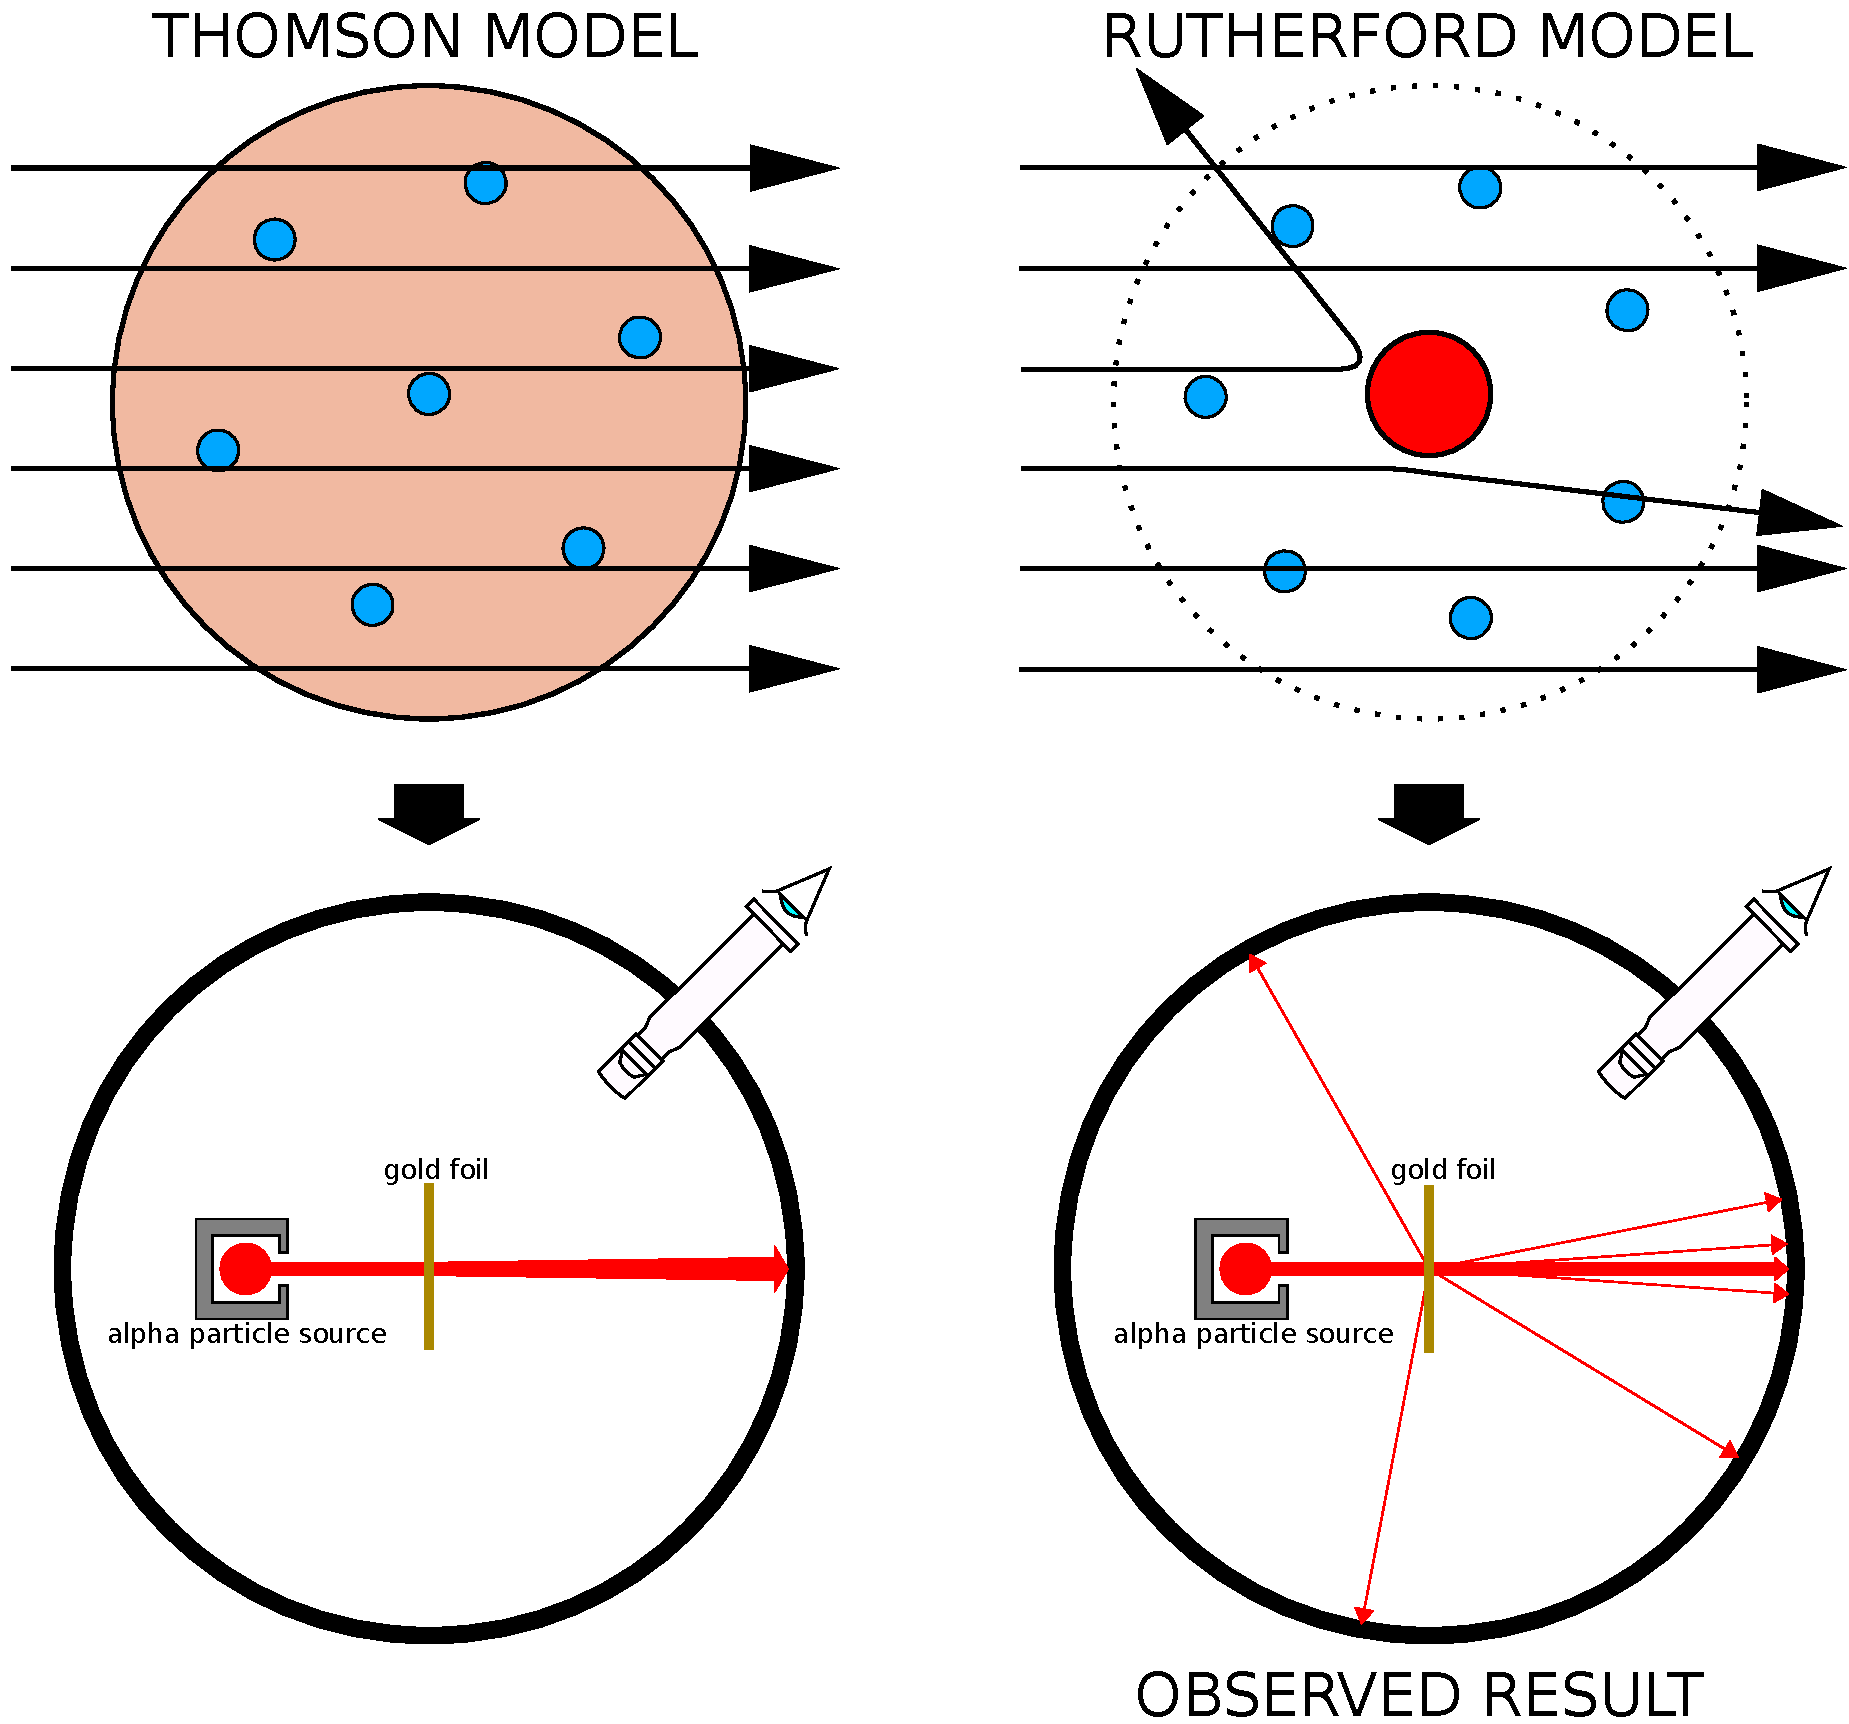
\includegraphics[width=0.7\linewidth]{fig/chapt2/Thomson_Rutherford_atoms.pdf}
		\caption{\label{fig:Atom_models} Through the gold foil experiment Rutherford could show that most of the mass of atoms was contained in a positively charged nucleus and could then propose a more accurate atomic model than that of Thomson.}
	\end{figure}
	
	The negative \textit{electron} would be the first to be discovered in 1897 by Thomson after 3 decades of research on cathode rays by proving that the electrification observed in an electroscope, as reported by Perrin, was due to the rays themselves and that they had to be composed of electrically charged particles. In 1900, Becquerel would show the \textit{beta rays} emitted by radium had the same charge over mass ratio than what measured by Thomson for cathode rays, pointing to eletrons as a constituant of atoms. In 1907, Rutherford and Royds showed that \textit{alpha} particles, once captured in a tube and subjected to an electric spark causing an electron avalanche, where heluim ions as they could combine with 2 electrons to form a $^4$He. This discovery was directly followed by the constraint of the atom structure in 1909 through the gold foil experiment in which the deflection angle of alpha particles fired at a very thin gold foil was measured and highlighted atoms where mainly empty with nearly all its mass contained into a tiny positively charged \textit{nucleus}. With these two observations, he could formulate the Rutherford model of the atom in 1911, shown together with the Thomson plum pudding model in Figure~\ref{fig:Atom_models}. The link in between atomic number and number of positive and negative charges contained into the atoms would fast be understood and the different kind of element transmutation appeared to be purely nuclear processes making clear that the electromagnetic nature of chemical transformation could not possibly change nuclei. Thus a new branch in physics appeared to study nuclei exclusively: the nuclear physics.
	
	Moreover, in 1913 quantum physics would be introduced into the atomic model by Bohr based on the asumptions of Plank to explain spectral lines, and other observed quantum effects. The same year, Moseley would confirm Borh's model and Debye would extend it by introducing eliptical orbits.
	
	By studying alpha emission and the product of their interaction with nitrogen gas, Rutherford reported in 1919 the very first nuclear reaction leading to the discovery that the hydrogen nucleus was composed of a single positively charged particle that was later baptised \textit{proton}. This idea came from 1815 Prout's hypothesis proposing that all atoms are composed of \textit{"protyles"} (i.e. hydrogen atoms). By using scintillation detectors, Rutherford could highlight typical hydrogen nuclei signature and understand that the impact of alpha particles with nitrogen would knock out an hydrogen nucleus and produce an oxygen 17, as explicited in Formula~\ref{eq:nuclear} and would then postulate that protons are building bricks of all elements.
	
	\begin{equation}
		\label{eq:nuclear}
		^{14}N + \alpha \rightarrow ^{17}O + p
	\end{equation}
	
	With this assumption and the discovery of isotopes together with Aston, elements with identical atomic number but different masses, Rutherford would propose that all elements' nuclei but hydrogen's are composed of both charged particles, protons, and of chargeless particles, which he called \textit{neutrons}, and that these neutral particles would help maintaining nuclei as one, as charged protons were likely to electrostatically repulse each other, and introduced the idea of a new force, a \textit{nuclear} force. Though the first idea concerning neutrons was a bond state of protons and electrons as it was known that the beta decay, emitting electrons, was taking place in the nucleus, it was then showed that such a model would hardly be possible due to Heisenberg's uncertainty principle and by the recently measured \textit{spin} of both protons and electrons. The spin, discovered through the study of the emission spectrum of alkali metals, would be understood as a "two-valued quantum degree of freedom" and formalized by Pauli and extended by Dirac, to take the relativist case into account. Measured to be $\frac{1}{2} \hbar$ for both, it was impossible to arrange an odd number of half integer spins and obtain a global nucleus spin that would be integer. Finally, in 1932, following the discovery of a new neutral radiation, Chadwick could discover the neutron as an uncharged particle with a mass similar to that of the proton whose half integer spin would reveal to be the solution to explain the nuclear spin.
	
	\subsubsection*{Development of the \acl{QED}}
	\label{chapt2:sssec:QED}
	
	Historically, the development of the quantum theory revolved around the question of emission and absorption of discrete amount of energy through light. Einstein used the initial intuition of Plank about the black-body radiation to develop in 1905 a model to explain the photoelectric effect in which light was described by discrete quanta now called \textit{photons}. For this model, Einstein introduced the concept of wave-particle duality as classical theory was not able to describe the phenomenon. With the new understanding of atoms and of their structure, classical theories also proved unable to explain atoms stability. Indeed, using classical mechanics, electrons orbiting aroung a nucleus should radiate an energy proportionnal to their angular momentum and thus loose energy through time and the spectrum of energy emission should then be continuous, but it was known since the \Th{19} century and the discovery of spectral lines that the emission spectrum of material was discrete.
	
	This was Bohr who first suggested that a quantum description of the atom was necessary in 1913. Using the correspondence principle stating that are large enough numbers the quantum calculations should give the same results than the classical theory, he proposed the very first quantum model of the hydrogen atom explaining the line spectrum by introducing the principal quantum number $n$ describing the electron shell. This model would then be improved by Sommerfeld that would quantize the z-component of the angular momentum, leading to a the second and third quantum numbers, or azimuthal and magnetic quantum number, $l$ and $m$ defining for the second the orbital angular momentum of the electrons on their shells and thus, the shape of the orbital, and for the third the available orbital on the subshell for each electron. Nevertheless, although the model was not only limited to sperical orbitals anymore, making the atom more realistic, the Zeeman effect couldn't be completely explained by just using $n$, $l$ and $m$. A solution would be brought after the discovery of Pauli in 1924, as Uhlenbeck, Goudsmit, and Kronig proposed in 1925 the idea of intrinsic rotation of the electron, introducing a new angular momentum vector associated to the particle itself, and not to the orbital, and associated to a new quantic number $s$, the \textit{spin} projection quantum number explaining the lift of degeneracy to an even number of energy levels.
	
	The introduction of the \textit{spin} happened 1 year after another attempt of improvement of the theory was made by De Broglie in his PhD thesis. The original formulation of the quantum theory only considered photons as energy quanta behaving as both waves and particles. De Broglie proposed that all matter are described by waves and that there momentum is proportional to the oscillation of quantized electromagnetic field oscillators. This interpretation was able to reproduce the previous version of the quantum energy levels by showing that the quantum condition involves an integer multiple of $2\pi$, as shown by Formula~\ref{eq:matterwave}.
	
	\begin{equation}
		\label{eq:matterwave}
		p = \hbar k \Leftrightarrow \int p dx = \hbar\int k dx = 2\pi\hbar n
	\end{equation}
	
	Although the intuition of De Broglie about the wave-particle duality of all matter, his interpretation was semiclassical and it's in 1926 that the first fully quantum mechanical wave-equation would be introduced by Schrödinger to describe electron-like particles, reproducing the previous semiclassical formulation without inconsistencies. This complexe equation describes the evolution of the wave function $\Psi$ of the quantum system, defined by it's position vector $\mathbf{r}$ and time $t$ as an energy conservation law, in which the hamiltonian of the system $\hat{H}$ is explicit, by solving the Equation~\ref{eq:schrodinger}.
	
	\begin{equation}
		\label{eq:schrodinger}
		i\hbar \frac{\partial}{\partial t} \vert \Psi(\mathbf{r},t)\rangle  = \hat{H} \vert \Psi(\mathbf{r},t)\rangle
	\end{equation}
	
	In 1927, Dirac would go further in his paper about emission and absorption of radiation by proposing a second quantization not only of the physical process at play but also of the electromagnetic field, providing the ingredients to the first formulation of \textit{\acf{QED}} and the description of photon emission by electrons dropping into a lower energy state in which the final number of particles is different than the initial one. To complete this model to the many-body wave functions of identical particles, Jordan included creation and annihilation operators for fields obeying Fermi-Dirac statistics leading to a model describing particles that would be referred to as \textit{fermions}. Nevertheless, in order to properly treat electromagnetism, the incorporation of the relativity theory developed by Einstein. Including gravity into quantum physics still is a challenge nowadays, but in 1928 Pauli and Jordan would show that special relativity's coordinate transformations could be applied to quantum fields as the field commutators were Lorentz invariant. Finally derived the same year, the Dirac equation, shown as Equation~\ref{eq:dirac}, similarly to Schrödinger's equation, is a single-particle equation but it incorporates special relativity in addition to quantum mechanics rules. It features the $4 \times 4$ gamma matrices $\gamma^\mu$ built using $2 \times 2$ Pauli matrices and unitary matrix, the 4-gradient $\partial_\mu$, the rest mass $m$ of any half integer spin massive particle described by the wave function $\psi(x,t)$, also called a Dirac spinor, and the speed of light $c$. In addition to perfectly reproduce the results obtained with quantum mechanics so far, it also provided with \textit{negative-energy solutions} that would later be interpreted as a new form of matter, \textit{antimatter} and give a theoretical justification to the Pauli equation that was phenomenologically constructed to account for the spin as in the non-relativistic limit, the Dirac equation is similar.
	
	\begin{equation}
		\label{eq:dirac}
		i\hbar \gamma^\mu\partial_\mu\psi - mc\psi = 0
	\end{equation}
	
	The successes of the QED was soon followed with theoretical problems as computations of any physical process involving photons and charged particles were showed to be only reliable at the first order of perturbation theory. At higher order of the theory, divergent contributions were appearing giving nonsensical results. Only two effects were contributing to these infinities.
	
	\begin{itemize}
		\item The self-energy of the electron (or positron), the energy that the particle has due its own interaction with its environment.
		\item The vacuum polarization, virtual electron–positron pairs produced by a background electromagnetic field in the vacuum which is not an "empty" space. These virtual pairs affect the charge and current distributions generated by the original electromagnetic field.
	\end{itemize}
	
	Solving this apparent problem was done by carefully defining the concepts of each observables, for example mass or charge, as these quantities are understood within the context of a non-interacting field equation, and that from the experiment point of view, they are abstractions as what is measured are "renormalized observables" shifted from there "bare" value by the interaction taking place in the measuring process. The infinities needed to be connected to corrections of mass and charge as those are fixed to finite values by experiement. This was the intuition of Bethe in 1947 who successfully computed the effect of such \textit{renormalization} in the non-relativist case. Fully covariant formulations of QED including renormalization was achieved by 1949 by Tomonaga, Schwinger, Feynman and Dyson and Feynman is now famous for his association of diagrams to the term of the scattering matrix, greatly simplifying the representation and computation of interactions as the diagrams directly corresponded the measurable physical processes and would then be used in every quantum field theories. With the resolution of infinities, QED had mostly reached its final form, being still today the most accurate physical theory and would serve as a model to build all other quantum field theories.
	
	\subsubsection*{Development of the quark model and \acl{QCD}}
	\label{chapt2:sssec:quark}
	
	To explain the nuclear force that holds \textit{nucleons} (protons and neutrons) together, Yukawa theoretically proposed in 1934 the existence of a force carrier called \textit{meson} due to it's predicted mass in the range in between the electron and nucleon masses. Discovered in 1936 by Anderson and Neddermeyer, and confirmed using bubble chambers in 1937 by Street and Stevenson, a first meson candidate was observed in the decay products of cosmic rays. Assuming it had the same electric charge than electrons and protons, this particle was observed to have a curvature due to magnetic field that was sharper than protons but smoother than electrons resulting in a mass in between that of electrons and protons. But its properties were not compatible with Yukawa's theory, which was emphasized by the discovery of a new candidate in 1947, again in cosmic ray products using photographic emulsions.
	
	This new candidate, although it had a similar mass than the already believed \textit{meson}, would rather decay into it. For distinction, the first candidate would then be renamed "\textit{mu meson}" when the second would be the "\textit{pi meson}". The \textit{mu meson} was behaving like a heavy electron and didn't participate in the strong interaction whereas the pion was believed to be the carrier of the nuclear interaction. This lead to classify the \textit{mu} in a new category of particles called \textit{leptons} together with the electron that shared similar properties and \textit{the} neutrino, and be renamed \textit{muon}. The \textit{pi meson} was finally found to be a triplet of particles: a positively charged, a negatively charged, and a neutral particle. The neutral \textit{pi meson} has been more difficult to identify as it wouldn't leave tracks on emulsions nor on bubble chambers and needed to be studied via it's decay products. It was ultimately identified in University of California's cyclotron in 1950 through the observation of its decay into 2 photons.
	
	Also discovered in 1947 but in cloud chamber photographs, the \textit{K meson} as also been an important step towards the establishment of the \acl{SM}. A triplet of particle, 2 charged and a neutral, with a mass roughly half that of a proton, were reported. These particles were baptised \textit{K meson} in contrast to the "light" \textit{pi} and \textit{mu} "L-mesons". The particularity of the \textit{K} were there very slow decays with a typical lifetime of the order of \Ord{-10}\si{s} much greater than the \Ord{-23}\si{s} of \textit{pi}-proton reactions. The concept of \textit{strangeness}, a new quantum number was then introduced by Pais as an attempt to explain this phenomenom as \textit{strange} particles appeared as a pair production of a strange and anti-strange particle.
	
	With the development of synchrotrons, the particle \textit{zoo} would grow to several dozens during the 1950s as higher energies were reachable through acceleration. In 1961, a first classification system, called Eightfold Way, was proposed by Gell-Mann and finding its roots in the Gell-Mann--Nishijima formula, which relates the electric charge $Q$, the third component of the isospin $I_3$, the \textit{baryon} number $B$ and the strangeness $S$, as explicited in Formula~\ref{eq:NNG}. The isospin was a quantum number introduced in 1932 to explain symmetries of the newly discovered neutron using representation theory of SU(2). The baryon number, was introduced by Nishijima as a quantum number for baryons, i.e. particles of the same family as nucleons. The mesons were classified in an octet and baryons of spin $\pm\frac{1}{2}$ and $\pm\frac{3}{2}$ were respectively classified into an octet and a decuplet, as shown in Figure~\ref{fig:Eightfold}. To complete the baryon decuplet, Gell-Mann predicted the existance of baryon $\Omega^-$ which would later be discovered in 1964.
	
	\begin{equation}
		\label{eq:NNG}
		Q = I_3 + \frac{1}{2}(B+S)
	\end{equation}
	
	\begin{figure}[H]
		\begin{subfigure}{\linewidth}
			\centering
			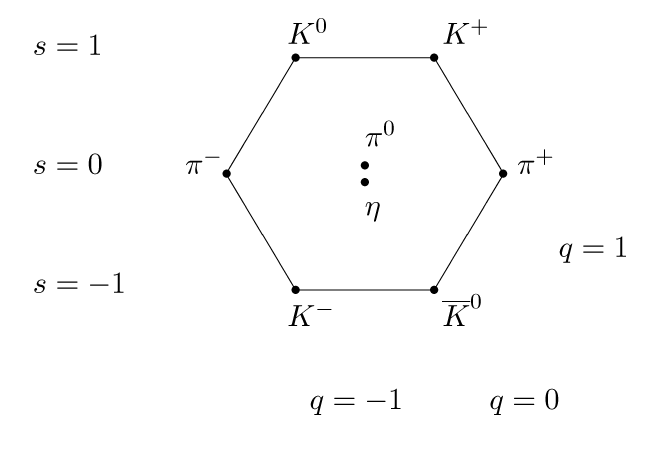
\includegraphics[width=0.4\linewidth]{fig/chapt2/Meson_octet.png}\\
			\caption{\label{fig:Eightfold:A}}
		\end{subfigure}
		\begin{subfigure}{0.5\linewidth}
			\centering
			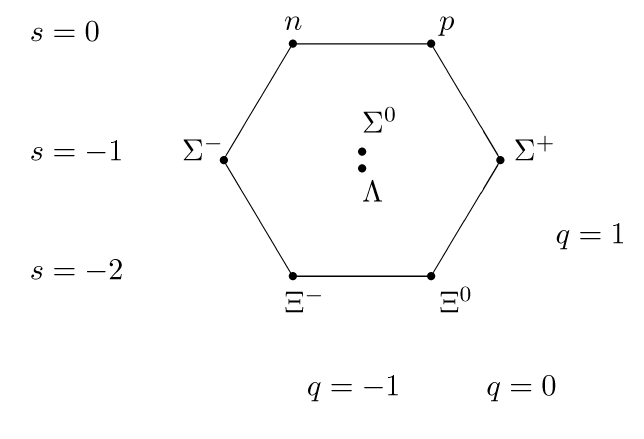
\includegraphics[width=0.8\linewidth]{fig/chapt2/Baryon_octet.png}
			\caption{\label{fig:Eightfold:B}}
		\end{subfigure}
		\begin{subfigure}{0.5\linewidth}
			\centering
			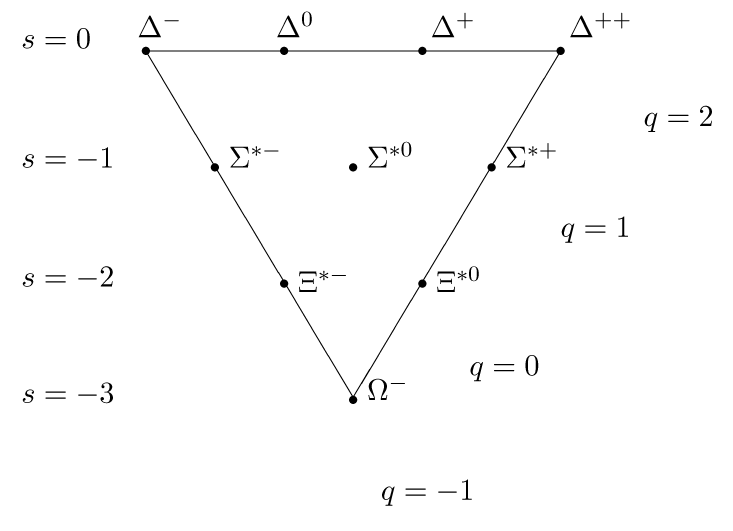
\includegraphics[width=0.8\linewidth]{fig/chapt2/Baryon_decuplet.png}
			\caption{\label{fig:Eightfold:C}}
		\end{subfigure}
		\caption{\label{fig:Eightfold} Figure~\ref{fig:Eightfold:A}: Meson octet. Figure~\ref{fig:Eightfold:B}: Baryon octet. Figure~\ref{fig:Eightfold:C}: Baryon decuplet.}
	\end{figure}
	
	Strong of this classification using an SU(3) flavor symmetry, Gell-Mann, and independently Zweig, would propose a full theoretical model in which \textit{hadrons} (strongly interacting particles, i.e. mesons and baryons) were not elementary particles anymore. They would rather be composed with 3 flavors of particles called \textit{quarks} and there anti-particles. The 3 flavors were called \textit{up}, \textit{down} and \textit{strange}. \textit{Up} and \textit{down} would be used to explain the nucleons and non-strange mesons, while \textit{strange} would come into the composition of hadrons showing strangeness. \textit{Up} and \textit{down} flavors would be discovered in 1968 thanks to the deep inelastic scattering experiments conducted at the \acf{SLAC}, and \textit{strange} could only be indirectly validated eventhough it provided a robust explanation to \textit{kaon} (K) and \textit{pion} ($\pi$). However, in the decade following the Gell-Mann-Zweig quark model proposition, several improvement to the model were brought, first by Glashow and Bjorken the same year that predicted the existence of a fourth quark flavor, the \textit{charm}, that would equalize the then known number of quarks and leptons and finally in 1973 by Kobayashi and Maskawa that would increase the number of quarks to 6 to explain the experimental observation of CP violation. These two quarks would been refered to as \textit{top} and \textit{bottom} for the first time in 1975. It's only after these additions to the quark model that finally the \textit{charm} would be discovered in 1974 at both SLAC and \acf{BNL}. A meson where the \textit{charm} was bond with an \textit{anti-charm}, called $J/\psi$, would help convince the physics community of the validity of the model. The \textit{top} would be discovered soon after in 1977 in Fermilab and indicate the existence of the \textit{bottom} that would resist to discovery until Fermilab's experiments CDF and D$\emptyset$ in 1995 due its very large mass and the energy needed to produce it.
	
	As remarked by Struminsky, the original quark model proposal composed of 3 quarks should possess an additional quantum number due to mesons such as $\Omega^-$ or $\Delta^{++}$. Indeed, these mesons are composed of 3 identical quarks, respectively 3 \textit{strange} and \textit{up} quark, with parallel spins, which should be forbidden by the exclusion principle. Independentle, Greenberg and Han-Nambu proposed an additional SU(3) degree of freedom possessed by the quarks, that would later be refered to as \textit{color charge gauge}, that could interact through \textit{gluons}, the gauge boson octet corresponding to this degree of freedom. Nevertheless, as observing free quarks proved to be impossible, two visions of the quarks were argued mainly due to the failures to observe these particles free to prove their existence. On one side, Gell-Mann proposed to see quarks as mathematical construct instead of real particles, as they are always confined, implying that quantum field theory would not describe entirely the strong interaction. Opposed to this vision, Feynman on the contrary argued that quarks were real particles, that he would call \textit{partons}, that should be described as all other particles by a distribution of position and momentum. The implications of quarks as point-like particles would be verified at SLAC and the concept of \textit{color} would be added to the quark model in 1973 by Fritzsch and Leutwyler together with Gell-Mann to propose a description of the strong interaction through the theory of \acf{QCD}. The discovery the same year of asymptotic freedom within the QCD by Groos, Politzer and Wilczek, allowed for very precise predictions thanks to the perturbation theory. Nowadays, the confinement of quarks is studied in experiments such as ALICE, through exploration of the quark-gluon plasma.
	
	\subsubsection*{The Weak interaction, spontaneous symmetry breaking, the Higgs mechanism and the Electroweak unification}
	\label{chapt2:sssec:HiggsEW}
	
	The weak interaction is the process that causes radioactive decays. Thanks to the neutron discovery, Fermi could explain in 1934 the beta radiations through the beta decay process in which the neutron decays into a proton by emitting an electron. Though the missing energy observed during this process triggered a huge debate about the apparent non conservation of energy, momentum and spin of the process, Fermi, as Pauli before him, proposed that the missing energy was due to a neutral not yet discovered particle that would then be baptised \textit{neutrino}. The impossibility to detect such a particle would leave some members of the scientific community sceptical, but hints of energy conservation and of the existence of the neutrino were provided by measuring the energy spectrum of electrons emitted through beta decay, as there was a strict limit on their energy. It's only 30 years later in 1953 that it would be discovered by the team of Cowan and Reines using the principle of inverse beta decay described through Formula~\ref{eq:invbeta}. The experiment consisted in placing water tanks sandwiched in between liquid scintillators near a nuclear reactor with an estimated neutrino flux of \Sci{5}{13}\siflux. However, in order to explain the absence of some reactions in the experiment of Cowan and Reines, and constraint the beta decay theory of Fermi and extend it to the case of the muon, Konopinski and Mahmoud proposed in 1953 that the muon decay would eject a particle similar to the neutrino and thus predicted the existence of a muon neutrino that would be different than the one involved in the beta decay, related to the electron. With this, the idea of lepton number would arise. The muon neutrino would successfully be detected in 1962 by lederman, Schwartz and Steinberger.
	
	\begin{equation}
		\label{eq:invbeta}
		\overline{\nu} + p \rightarrow n + e^+
	\end{equation}
	
	The theory could not be valid though as the probability of interaction, called cross-section, would have been increasing without bond with the square of the energy. Fermi assumed in a two vector current coupling but Lee and Yang noted that an axial current could appear and would violate parity. The experiment of Wu in 1956 would confirm the parity violation and Gamov and Teller would try to account for it by describing Fermi's interaction through allowed (parity-violating) and superallowed (parity-conserving) decays. But the success of QED as a quantum field theory would spark the development of such a theory to describe the weak interaction.
	
	As previously discussed, the great success of QED was built on an underlying symmetry, interpreted as a gauge invariance so that the effect of the force is the same in all space-time coordinates, and of the possibility to renormalize it in order to absorb the infinites. Independently in 1958, Glashow, and Salam and Ward used 1957 Schwinger ideas about vector intermediary for the decay processes, could find a way to unite both the electromagnetic and weak interaction into a gauge theory involving 4 gauge bosons, 3 of which were massive and carried out the weak interaction and a massless boson carrying the electromagnetic interaction. Among the 3 massive bosons, 2 were charged and 1 was neutral, similarly to the previously theorized \textit{pi meson} vector of the Yukawa model and all have a mass much greater than nucleons and thus a very short life time implying a finite very short range contrary to the contact interaction originally proposed by Fermi.
	
	Breakthrough in other fields of physics contributed in giving theoretical support and interpretation to the unified electroweak theory. The stepping stone would be the use of spontaneous symmetry breaking that was inspired to Nambu at the end of the 1950s following the development of the BCS superconductivity mechanism in 1957. Cooper had shown that BCS pairs, pairs of electrons bound together at low temperature, could have lower energy than the Fermi energy and where responsible for superconductivity. This lead to the discovery of Goldstone-Nambu bosons as a result of the spontaneous breaking of the chiral symmetry in a theory describing nucleons and mesons developped by Nambu and Jona-Lasinio in 1961, and now understood as a low-ebergy approximation of QCD. Simmilarly to mechanism of energy gap appearance in superconductivity, the nucleon mass is suggested to the result of a self-energy of a fermion field and is studied through a four-fermion interaction in which, as a consequence of the symmetry, bound states of nucleon-antinucleon pairs appear and can be regarded as virtual pions. Though the symmetry is maintained in the equations, the ground state is not preserved. Goldstone would later the same year show that the bound states corresponds to spinless bosons with zero mass.
	
	Although the model in itself didn't revolutionize particle physics, spontaneous symmetry breaking would be generalized to quantum field theories. As all fundamental interactions are described using gauge theories based on underlying symmetries, processes such as the chiral symmetry breaking would be introduced soon after the publication of Nambu and Jona-Lasinio. In 1962, Anderson, following an idea of Schwinger who suggested that zero-mass vector bosons were not necessarily required to describe the conservation of baryons contrary to the bosons emerging from chiral symmetry breaking, discussed the implications of spontaneous symmetry breaking in particles physics. A model was finally independently built in 1964 by Brout and Englert, Higgs, and Guralnik, Hagen, and Kibble, who discovered that combining an additional field into a gauge theory in order to break the symmetry, the resulting gauge bosons acquire a nonzero mass. Moreover, Higgs stated that this implied the existence of at least one new massive, i.e. self-interacting, scalar boson, that are now known as \textit{Higgs bosons} corresponding to this additional field. The Higgs mechanism today specifically refers to the process through which the gauge bosons of the weak interaction acquire mass. In 1968, Weinberg could point to the Higgs mechanism to integrate a Higgs field into a new version of the electroweak theory in which the spontaneous symmetry breaking mechanism of the Higgs field would explicitely explain the masses of the weak interaction gauge bosons and the zero-mass of photons.
	
	\subsection{Construction and test of the model}
	\label{chapt2:ssec:model}
	
	
	
	\subsection{Investigating the TeV scale}
	\label{chapt2:ssec:TeV}

\section{The \acl{LHC} \& the \acl{CMS}}
\label{chapt2:sec:LHC-CMS}

	Throughout its history, CERN has played a leading role in high energy particle physics. Large regional facilities such as CERN were thought after the second world war in an attempt to increase international scientific collaboration and allows scientists to share the forever increasing costs of experiment facilties required due to the need for increasing the energy in the center of mass to deeper probe matter. The construction of the first accelerators at the end of the 50s, the \acf{SC} and the \acf{PS}, was directly followed by the first observation of antinuclei in 1965~\cite{MASSAM1965}. Strong from the experience of the \acf{ISR}, the very first proton-proton collider that showed hints that protons are not elementary particles, the \acf{SPS} was built in the 70s to investigate the structure of protons, the preference for matter over antimatter, the state of matter in the early universe or exotic particles, and lead to the discovery in 1983 of the W and Z bosons~\cite{UA1W1983,UA2W1983,UA1Z1983,UA2Z1983}. These newly discovered particles and the electroweak intereaction would then be studied in details by the \acf{LEP} collider that will help to prove in 1989 that there only are three generations of elementary particles~\cite{ALEPH1989}. The LEP would then be dismantled in 2000 to allow for the LHC to be constructed in the existing tunnel.

	\subsection{LHC, the most powerful particle accelerator}
	\label{chapt2:ssec:LHC}
	
	The LHC has always been considered as an option to the future of CERN. At the moment of the construction of the LEP beneath the border between France and Switzerland, the tunnel was built in order to accomodate what would be a \acl{LHC} with a dipole field of \SI{10}{T} and a beam energy in between 8 and \SI{9}{TeV}~\cite{ANNUALREPORT1984} directly followed in 1985 with the creation of a 'Working Group on the Scientific and Technological Future of CERN' to investigate such a collider~\cite{ANNUALREPORT1985}. The decision was finally taken almost 10 years later, in 1994, to construct the LHC in the LEP tunnel~\cite{ANNUALREPORT1994} and the approval of the 4 main experiments that would take place at the 4 interaction points would come in 1997~\cite{ANNUALREPORT1997} and 1998~\cite{ANNUALREPORT1998}:
	
	\begin{itemize}
		\item[•] ALICE~\cite{ALICELOI} has been designed in the purpose of studying quark-gluon plasma that is believed to have been a state of matter that existed in the very first moment of the universe.
		\item[•] ATLAS~\cite{ATLASLOI} and CMS~\cite{CMSLOI} are general purpose experiements that have been designed with the goal of continuing the exploration of the Standard Model and investigate new physics.
		\item[•] LHCb~\cite{LHCBLOI} has been designed to investigate the preference of matter over antimatter in the universe through the CP violation.
	\end{itemize}
	
	These large scale experiments, as well as the full CERN accelerator complex, are displayed on Figure~\ref{fig:CERNComplex}.

	\begin{figure}[H]
		\centering
		\hspace*{-0.1\linewidth}
		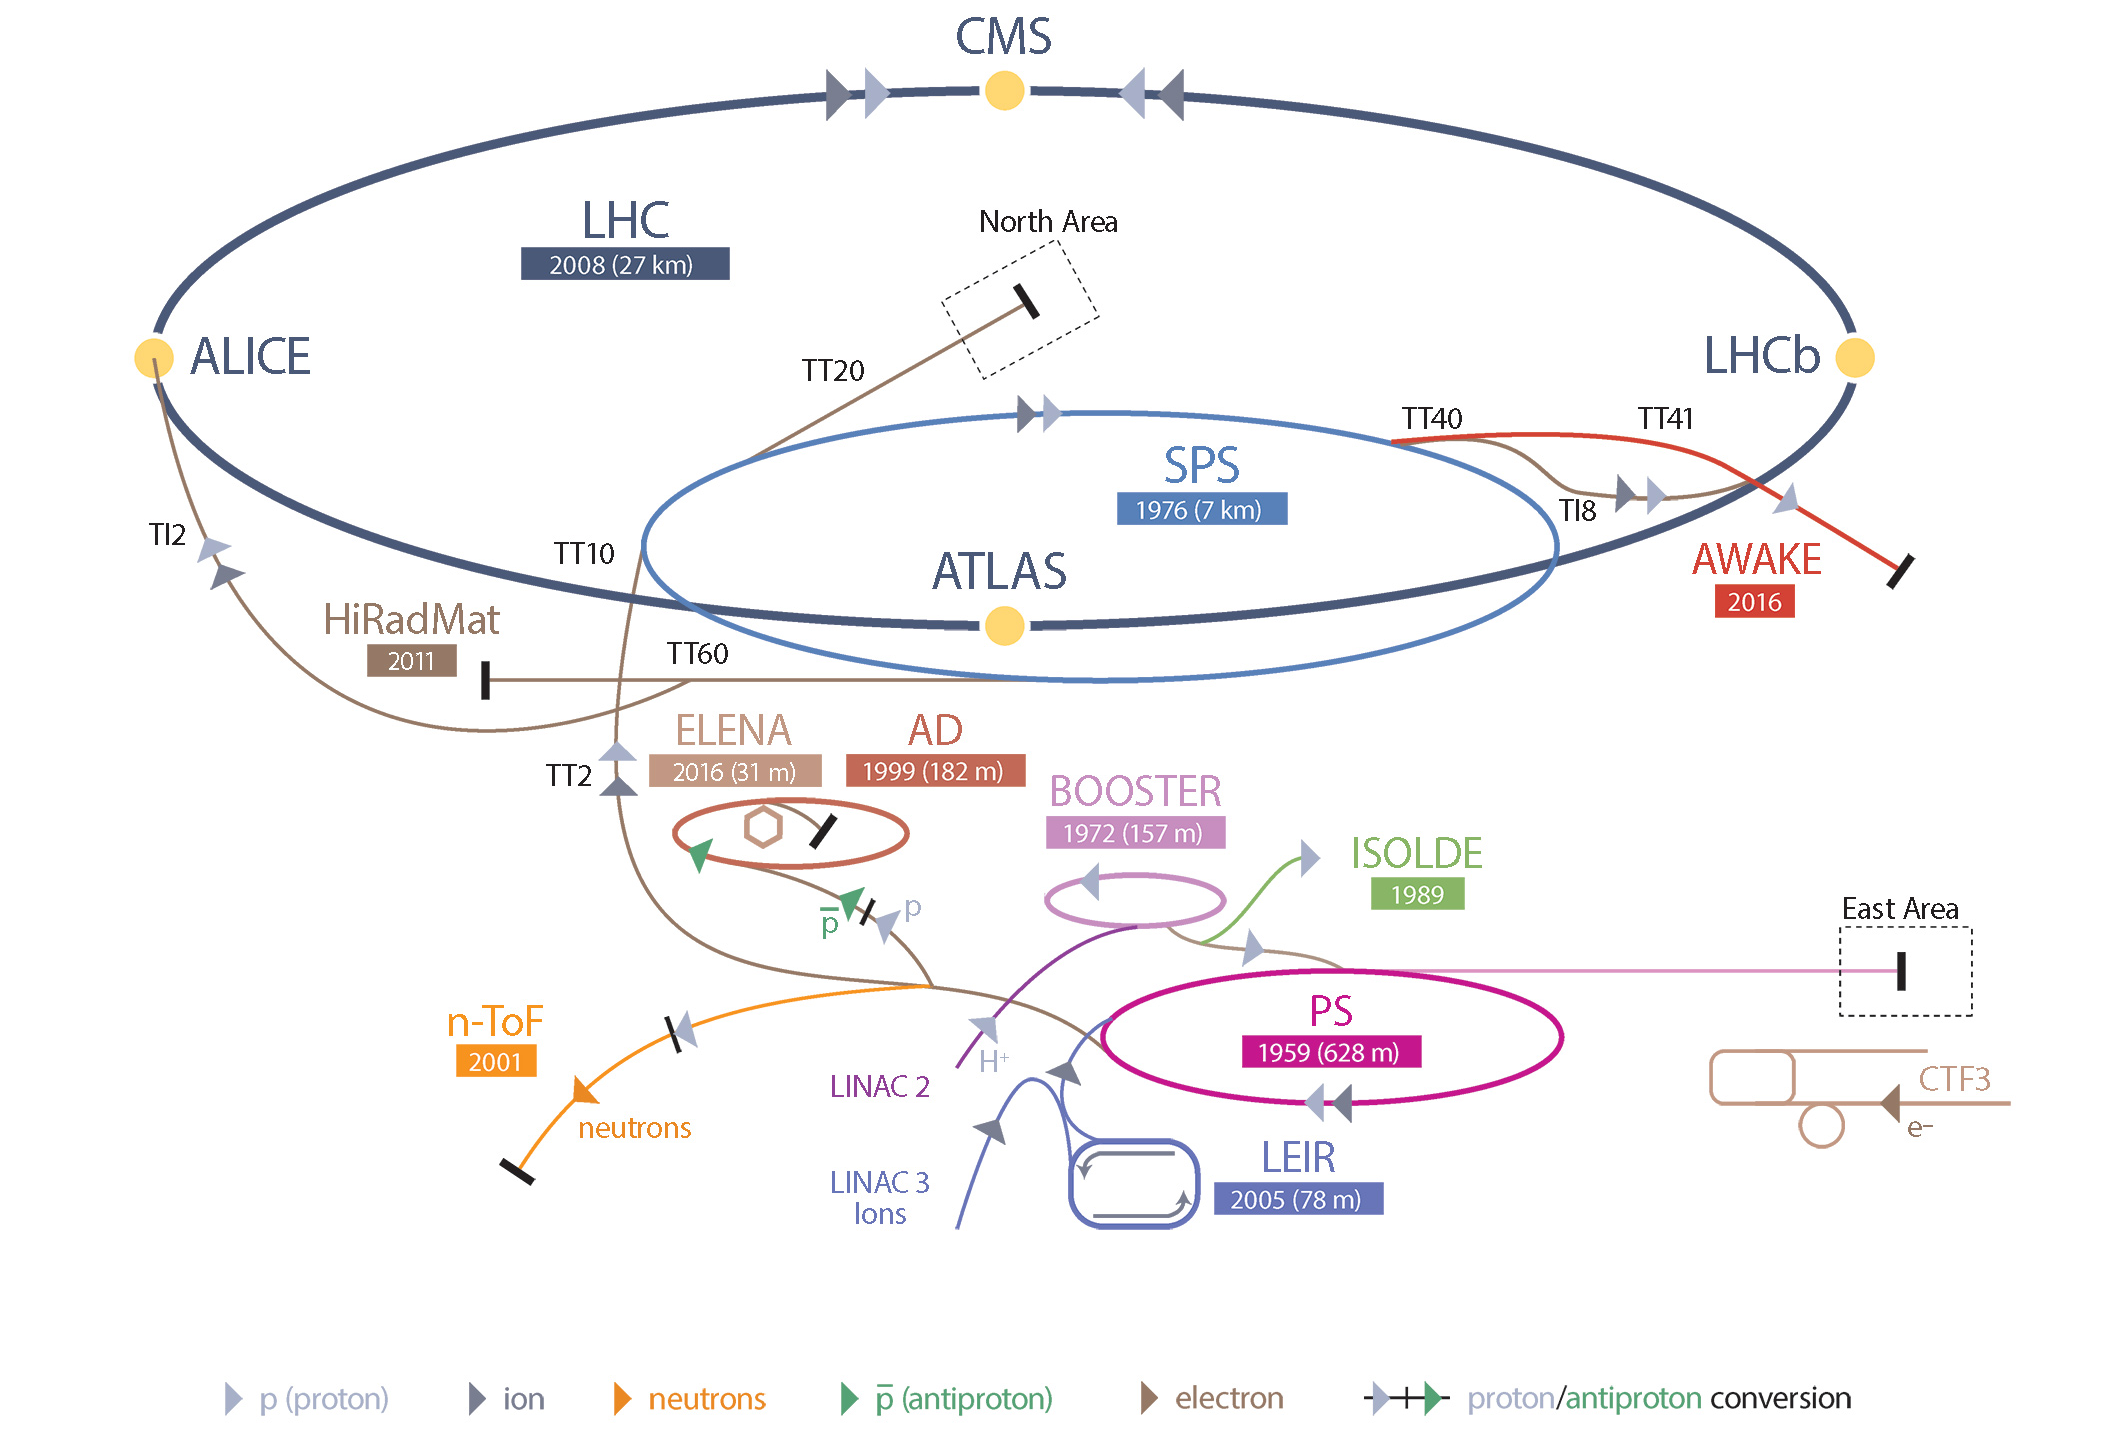
\includegraphics[width=1.2\linewidth]{fig/chapt2/CERN_Accelerator_Complex.png}
		\caption{\label{fig:CERNComplex} CERN accelerator complex.}
	\end{figure}
	
	The LHC is a \SI{27}{km} long hadron collider and the most powerful accelerator used for particle physics since 2008~\cite{LHC2008}. The LHC was originally designed to collide protons at a center-of-mass energy of \SI{14}{TeV} and luminosity of $10^{34}$ \si{cm^{-2}s^{-1}}, as well as $Pb$ ions at a center-of-mass energy of \SI{2.8}{TeV/A} with a peak luminosity of $10^{27}$ \si{cm^{-2}s^{-1}}. Run 1 of LHC, when the center-of-mass energy only was half of the nominal LHC energy, was enough for both CMS and ATLAS to discover the Higgs boson~\cite{HIGGS2015} and for LHCb to discover pentaquarks~\cite{PENTAQUARK2015} and confirm the existance of tetraquarks~\cite{TETRAQUARK2017}. Nevertheless, after the \acf{LS3} (2024-2026), the accelerator will be in the so called \acf{HL-LHC} configuration~\cite{HLLHC2017}, increasing its instantaneous luminosity to $10^{35}$ \si{cm^{-2}s^{-1}} for $pp$ collisions and to $4.5\times 10^{27}$ \si{cm^{-2}s^{-1}}, boosting the discovery potential of the LHC.
	
		\subsubsection{Particle acceleration}
		\label{chapt2:sssec:acceleration}
	
	The LHC is the last of a long series of accelerating devices. Before being accelerated by the LHC, the particles need to pass through different acceleration stages. All these acceleration stages are visible on Figure~\ref{fig:CERNComplex} and pictures of the accelerators are showed in Figure~\ref{fig:CERNAccelerators}.\\
	
	The story of accelerated protons at CERN starts with a bottle of hydrogen gas injected into the source chamber of the linear particle accelerator \textit{LINAC 2} 2 in which a strong electric field strips the electron off the hygroden molecules only to keep their nuclei, the protons. The cylindrical conductors, alternatively positively or negatively charged by radiofrequency cavities, accelerate protons by pushing them from behing and pulling them from the front and ultimately give them an energy of \SI{50}{MeV}, increasing their mass by 5\% in the process.\\
	
	When exiting the LINAC 2, the protons are divided into 4 bunches and injected into the 4 superimposed synchrotron rings of the \textit{Booster} where they are then accelerated to reach an energy of \SI{1.4}{GeV} before being injected into the \textit{PS}. Before the Booster was operational in 1972, the protons were directly injected into the PS from the LINAC 2 but the low injection energy limited the amount of protons that could be accelerated at once by the PS. With the Booster, the PS accepts approximately 100 times more particles.\\
	
	The 4 proton bunches are thus sent as one to the PS where their energy eventually reaches \SI{26}{GeV}. Since the 70s, the main goal of this \SI{628}{m} circumference synchrotron has been to supply other machines with accelerated particles. Nowadays, not only the PS accelerates protons, it also accelerates heavy ions from the \textit{\acf{LEIR}}. Indeed, the LHC experiments are not only designed to study $pp$-collinsions but also $Pb$-collisions. Lead is first injected into the dedicated linear collider \textit{LINAC 3}, that accelerate the ions using the same principle than LINAC 2. Electrons are striped off the lead ions all along the acceleration process and eventually, only bare nuclei are injected in the LEIR whose goal is to transform the long ion pulses received into short dense bunches for LHC. Ions injected and stored in the PS were aceelerated by the LEIR from \SI{4.2}{MeV} to \SI{72}{MeV}.\\
	
	Directly following the PS, is finally the last acceleration stage before the LHC, the \SI{7}{km} long \textit{SPS}. The SPS accelerates the protons to \SI{450}{GeV} and inject proton in both LHC accelerator rings that will increase their energy up to \SI{7}{TeV}. When the LHC runs with heavy lead ions for ALICE and LHCb, ions are injected and accelerated to reach the energy of \SI{2.8}{TeV/A}.

	\begin{figure}[H]
		\centering
		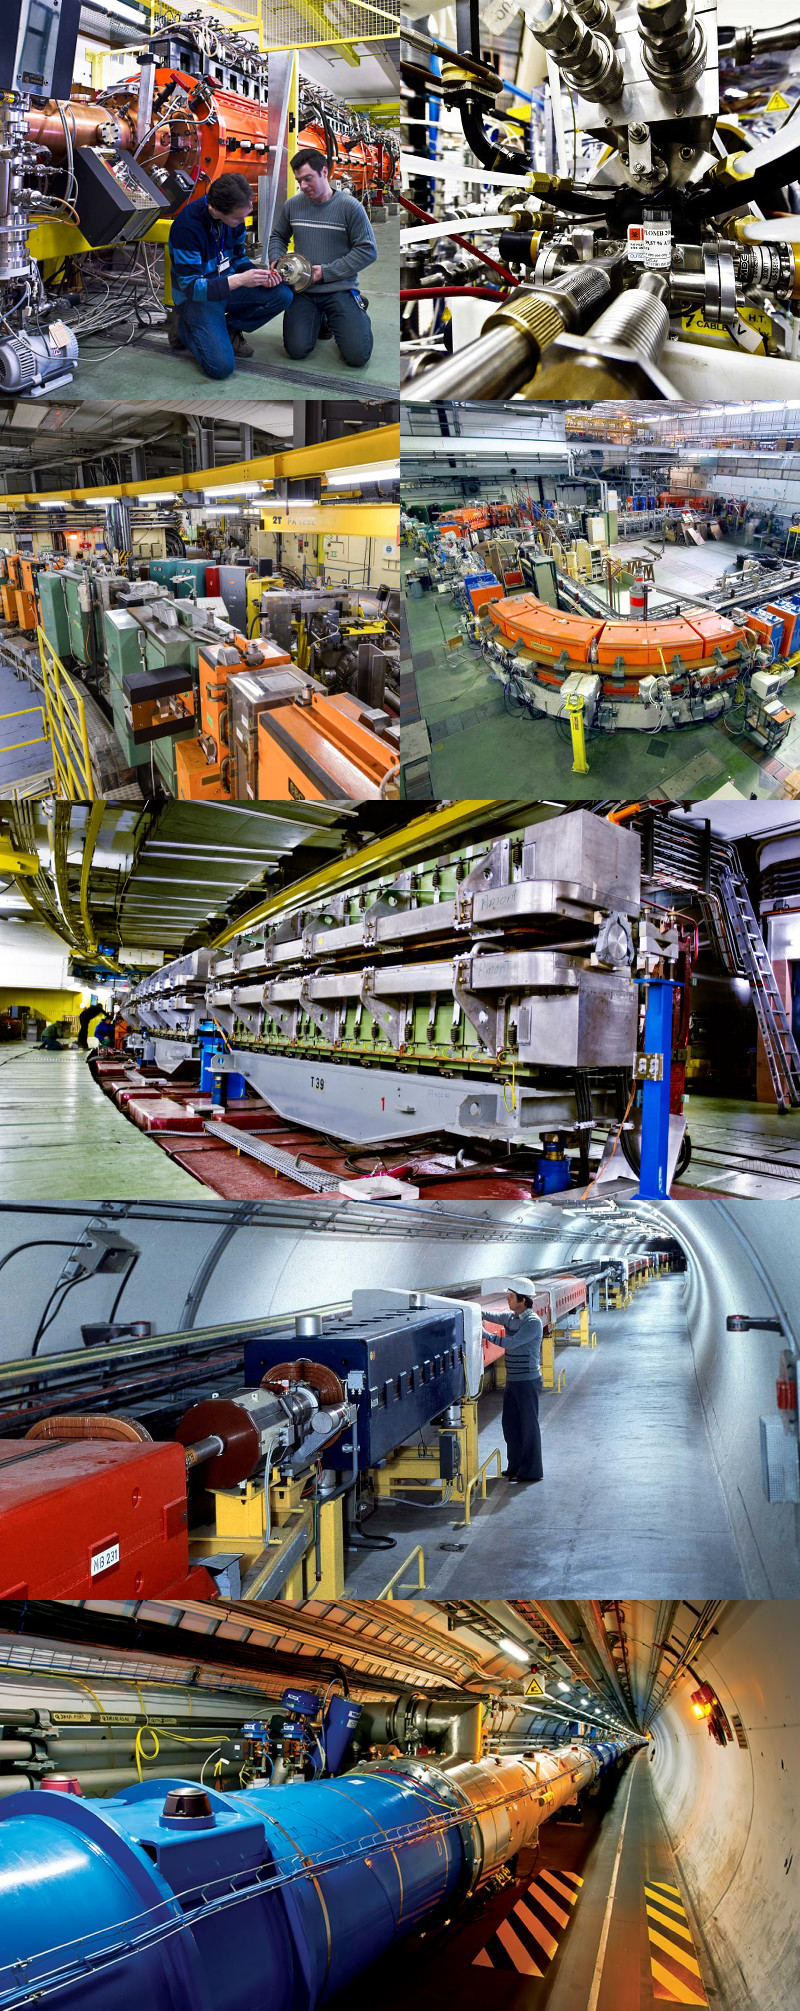
\includegraphics[width=0.5\linewidth]{fig/chapt2/CERN-accelerators.jpg}
		\caption{\label{fig:CERNAccelerators} Pictures of the different accelerators. From top to bottom: first the LINAC 2 and the $Pb$ source of LINAC 3. Then the Booster and the LEIR. Finally, the PS, the SPS and the LHC.}
	\end{figure}
	
	The LHC beams are not continuous and are rather organised in bunch of paticles. When in $pp$-collision mode, the beams are composed of 2808 bunches of $1.15 \times 10^{11}$ protons separated by \SI{25}{ns}. When in $Pb$ collision mode, the 592 $Pb$ bunches are on the contrary composed of $2.2 \times 10^8$ ions separated by \SI{100}{ns}. The two parrallel proton beams of the LHC are contained in a single twin-bore magnet due to the space restriction in the LEP tunnel. Indeed, building 2 completely separate accelerator rings next to each other was impossible. The dipoles of the 1232 twin-bore magnets are showed in Figure~\ref{fig:LHCDipole} alongside the magnetic field generated along the dipole section to accelerate the particles. The dipoles generate a nominal field of \SI{8.33}{T}, needed to give protons and lead nucleons their nominal energy. Some 392 quadrupoles, presented in Figure~\ref{fig:LHCQuadrupole}, are also used to focus to the beams, as well as other multipoles to correct smaller imperfections.
	
	\begin{figure}[H]
		\begin{subfigure}{0.5\linewidth}
			\centering
			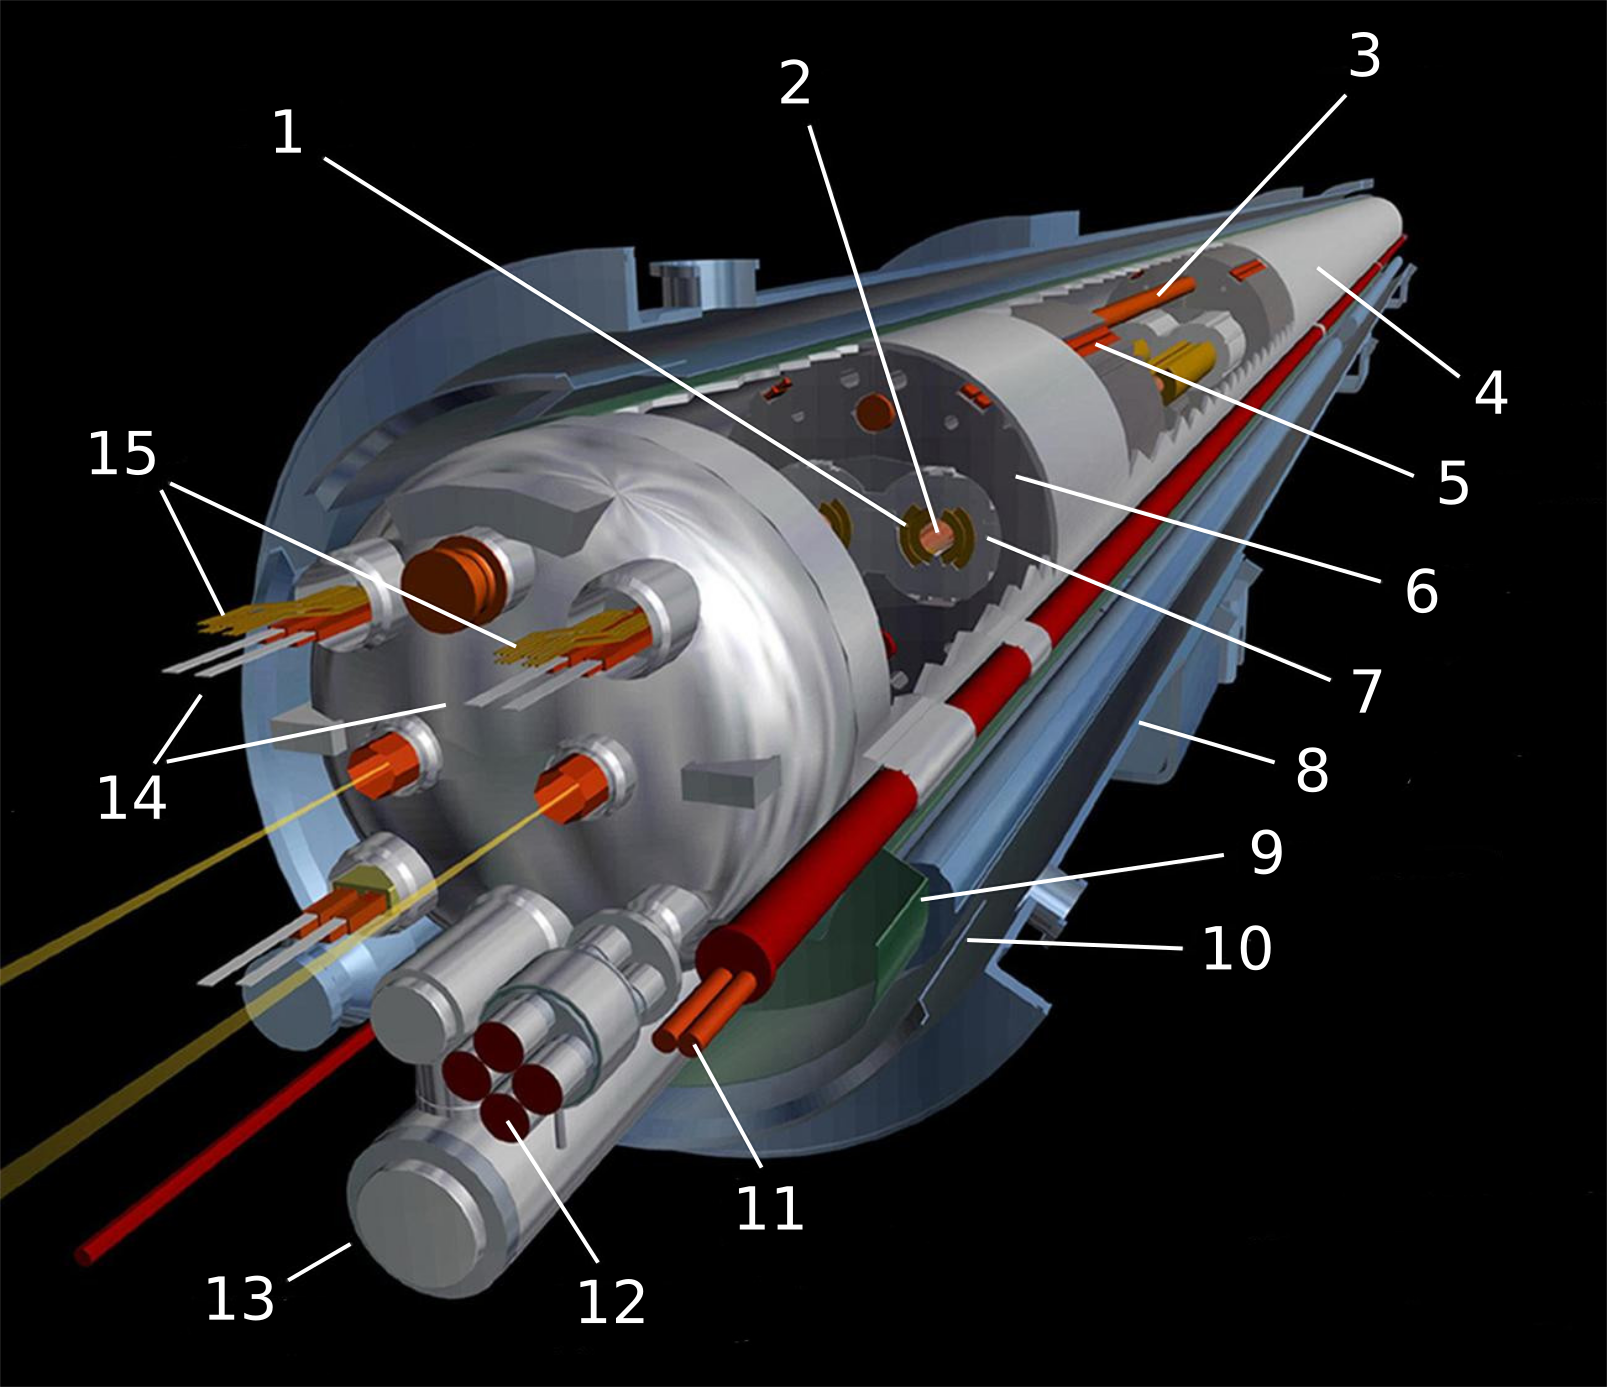
\includegraphics[height = 4cm]{fig/chapt2/LHC-dipole.png}
			\caption{\label{fig:LHCDipole:A}}
		\end{subfigure}
		\begin{subfigure}{0.5\linewidth}
			\centering
			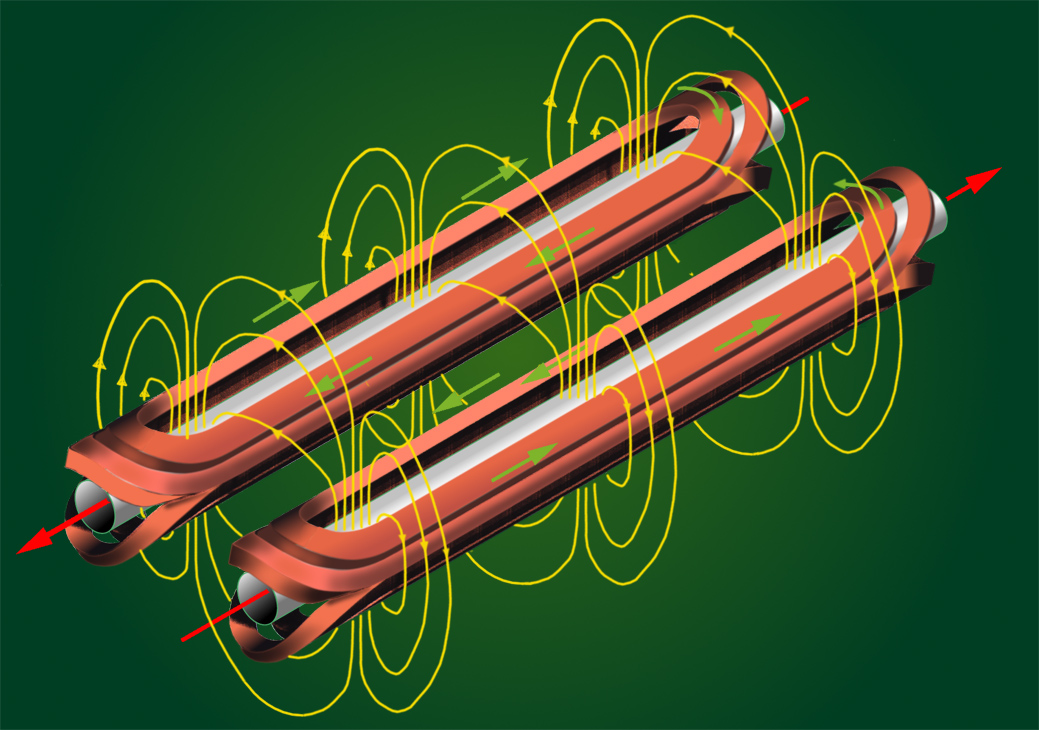
\includegraphics[height = 4cm]{fig/chapt2/LHC-dipole-field.jpg}
			\caption{\label{fig:LHCDipole:B}}
		\end{subfigure}
		\caption{\label{fig:LHCDipole} Figure~\ref{fig:LHCDipole:A}: schematics of the LHC cryodipoles. 1: Superconducting Coils, 2: Beam pipe, 3: Heat exchanger Pipe, 4: Helium-II Vessel, 5: Superconducting Bus-bar, 6: Iron Yoke, 7: Non-Magnetic Collars, 8: Vacuum Vessel, 9: Radiation Screen, 10: Thermal Shield, 11: Auxiliary Bus-bar Tube, 12: Instrumentation Feed Throughs, 13: Protection Diode, 14: Quadrupole Bus-bars, 15: Spool Piece Bus-bars. Figure~\ref{fig:LHCDipole:B}: magnetic field and resulting motion force applied on the beam particles.}
	\end{figure}
	
	\begin{figure}[H]
		\begin{subfigure}{0.5\linewidth}
			\centering
			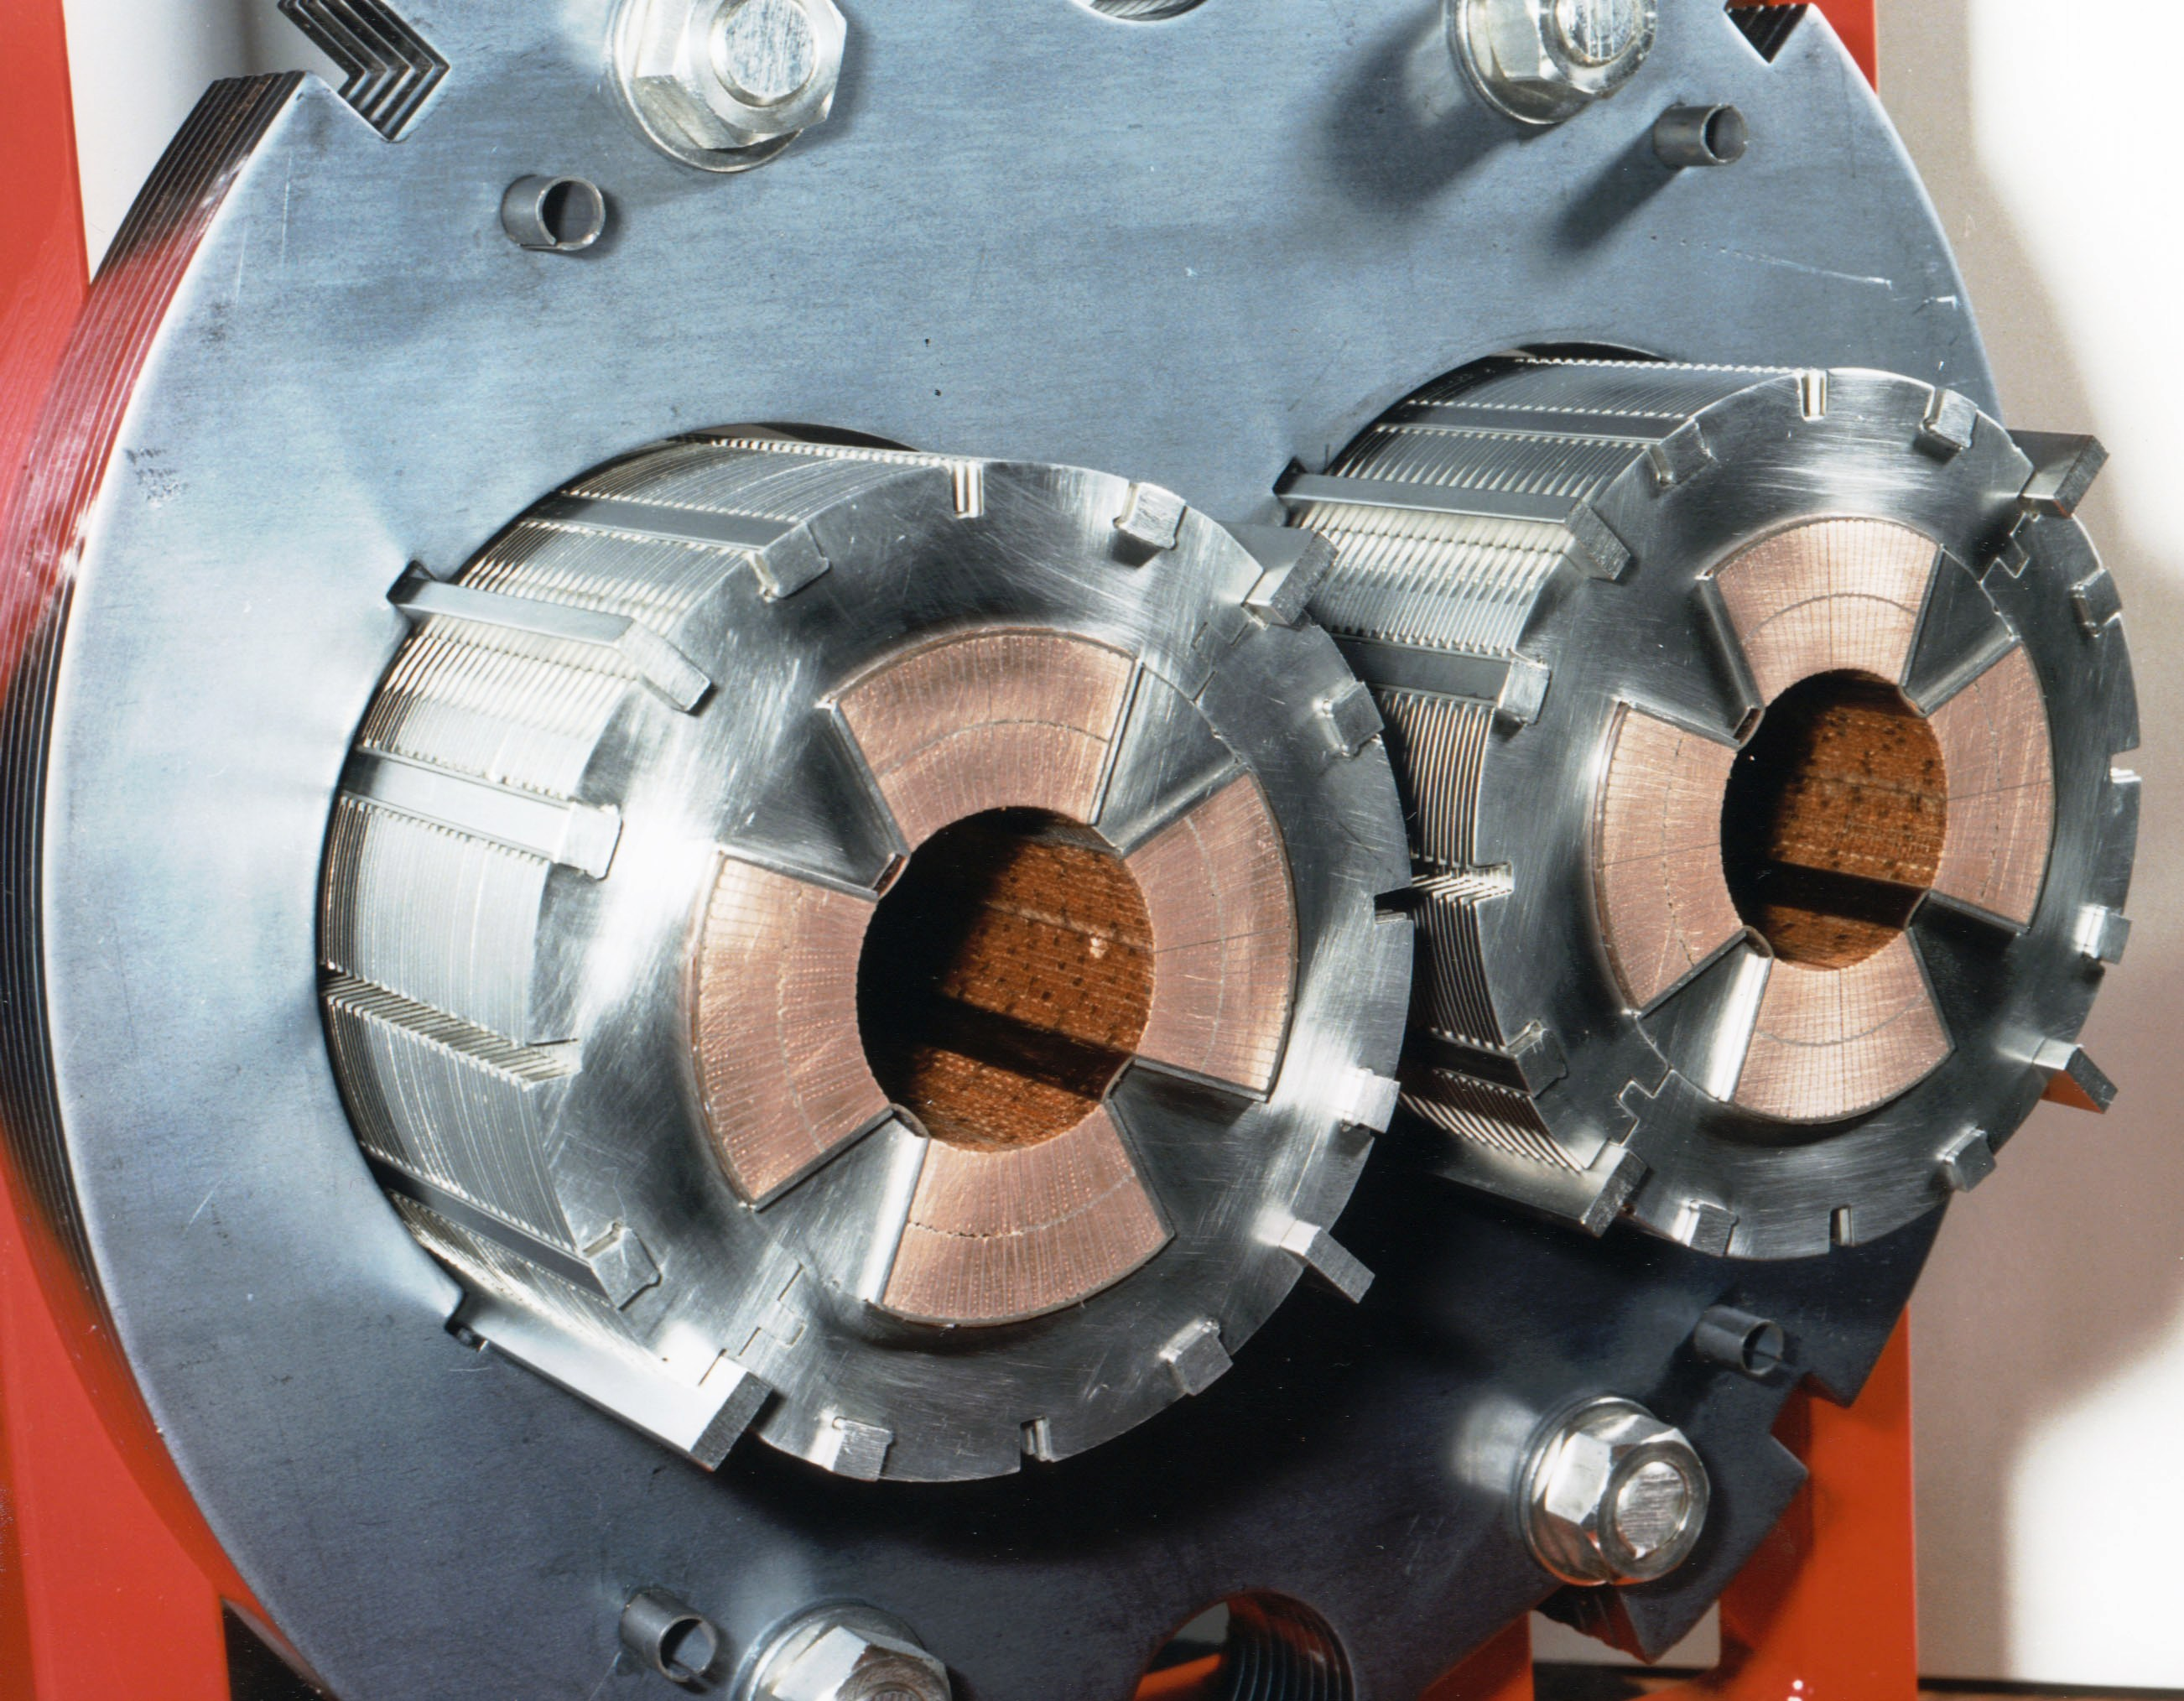
\includegraphics[height = 4cm]{fig/chapt2/LHC-quadrupole.jpg}
			\caption{\label{fig:LHCQuadrupole:A}}
		\end{subfigure}
		\begin{subfigure}{0.5\linewidth}
			\centering
			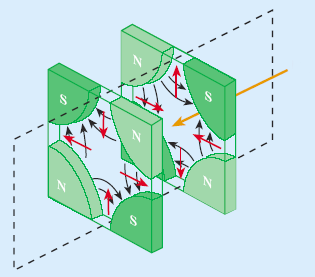
\includegraphics[height = 4cm]{fig/chapt2/LHC-quadrupole-field.png}
			\caption{\label{fig:LHCQuadrupole:B}}
		\end{subfigure}
		\caption{\label{fig:LHCQuadrupole} Figure~\ref{fig:LHCQuadrupole:A}: picture of the LHC quadrupoles. Figure~\ref{fig:LHCQuadrupole:B}: magnetic fields and resulting focussing force applied on the beam by 2 consecutive quadrupoles.}
	\end{figure}
	
		\subsubsection{LHC discoveries and LHC physics program}
		\label{chapt2:sssec:discovery}
		
	The very first proton beam successfully circulated in the LHC in September 2008 directly followed by an incident leading to mechanical damage that would delay the LHC program for a year until November 2009.
	
		\subsubsection{\acl{HL-LHC}}
		\label{chapt2:sssec:HL-LHC}

	\subsection{CMS, a multipurpose experiment}
	\label{chapt2:ssec:CMS}

\section{Muon Phase-II Upgrade}
\label{chapt2:sec:phase-2}

After the more than two years lasting \acf{LS1}, the \acf{LHC} delivered its very first Run-II proton-proton collisions early 2015. LS1 gave the opportunity to the LHC and to the its experiments to undergo upgrades. The accelerator is now providing collisions at center-of-mass energy of \SI{13}{TeV} and bunch crossing rate of \SI{40}{MHz}, with a peak luminosity exceeding its design value. During the first and upcoming second LHC Long Shutdown, the \acf{CMS} detector is also undergoing a number of upgrades to maintain a high system performance~\cite{MUONTDR}.

From the LHC Phase-2 or \acf{HL-LHC} period onwards, i.e. past the \acf{LS3}, the performance degradation due to integrated radiation as well as the average number of inelastic collisions per bunch crossing, or pileup, will rise substantially and become a major challenge for the LHC experiments, like CMS that are forced to address an upgrade program for Phase-II~\cite{PHASEIITP}. Simulations of the expected distribution of absorbed dose in the CMS detector under HL-LHC conditions, show in figure~\ref{fig:Dose} that detectors placed close to the beamline will have to withstand high irradiation, the radiation dose being of the order of a few tens of\si{Gy}.

\begin{figure}[H]
	\centering
	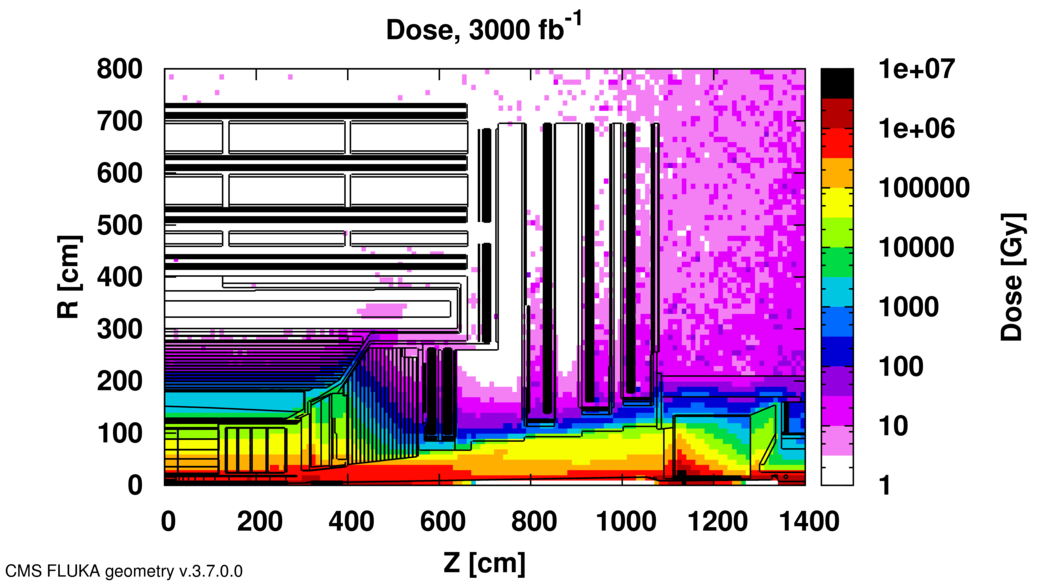
\includegraphics[width=0.7\textwidth]{fig/chapt2/HL-LHC-Dose.png}
	\caption{\label{fig:Dose} Absorbed dose in the CMS cavern after an integrated luminosity of \SI{3000}{\femto\per\barn}. R is the transverse distance from the beamline and Z is the distance along the beamline from the Interaction Point at Z=0.}
\end{figure}

The measurement of small production cross-section and/or decay branching ratio processes, such as the Higgs boson coupling to charge leptons or the $B_s \longrightarrow \mu^+\mu^-$ decay, is of major interest and specific upgrades in the forward regions of the detector will be required to maximize the physics acceptance on the largest possible solid angle. To ensure proper trigger performance within the present coverage, the muon system will be completed with new chambers. In figure~\ref{fig:Quadrant} one can see that the existing \acfp{CSC} will be completed by \acfp{GEM} and \acfp{RPC} in the pseudo-rapidity region $1.6<\vert\eta\vert<2.4$ to complete its redundancy as originally scheduled in the CMS Technical Proposal~\cite{CMSTP}.

\begin{figure}[H]
	\centering
	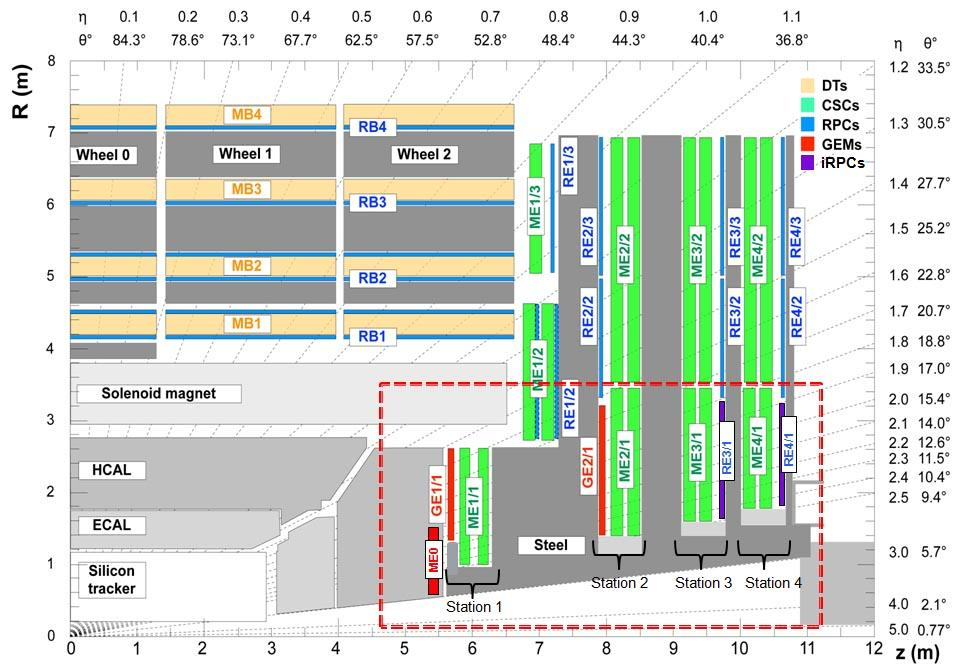
\includegraphics[width=0.7\textwidth]{fig/chapt2/MuonUpgrade-Plans.jpg}
	\caption{\label{fig:Quadrant} A quadrant of the muon system, showing DTs (yellow), RPCs (light blue), and CSCs (green). The locations of new forward muon detectors for Phase-II are contained within the dashed box and indicated in red for GEM stations (ME0, GE1/1, and GE2/1) and dark blue for improved RPC (iRPC) stations (RE3/1 and RE4/1).}
\end{figure}

RPCs are used by the CMS first level trigger for their good timing performances. Indeed, a very good bunch crossing identification can be obtained with the present CMS RPC system, given their fast response of the order of \SI{1}{ns}. In order to contribute to the precision of muon momentum measurements, muon chambers should have a spatial resolution less or comparable to the contribution of multiple scattering~\cite{MUONTDR}. Most of the plausible physics is covered only considering muons with $p_T<$\SI{100}{GeV} thus, in order to match CMS requirements, a spatial resolution of $\mathcal{O}$(few $\mathrm{mm}$) the proposed new RPC stations, as shown by the simulation in figure~\ref{fig:MultiScat}. According to preliminary designs, RE3/1 and RE4/1 readout pitch will be comprised between 3 and \SI{6}{mm} and 5 $\eta$-partitions could be considered.

\begin{figure}[H]
	\centering
	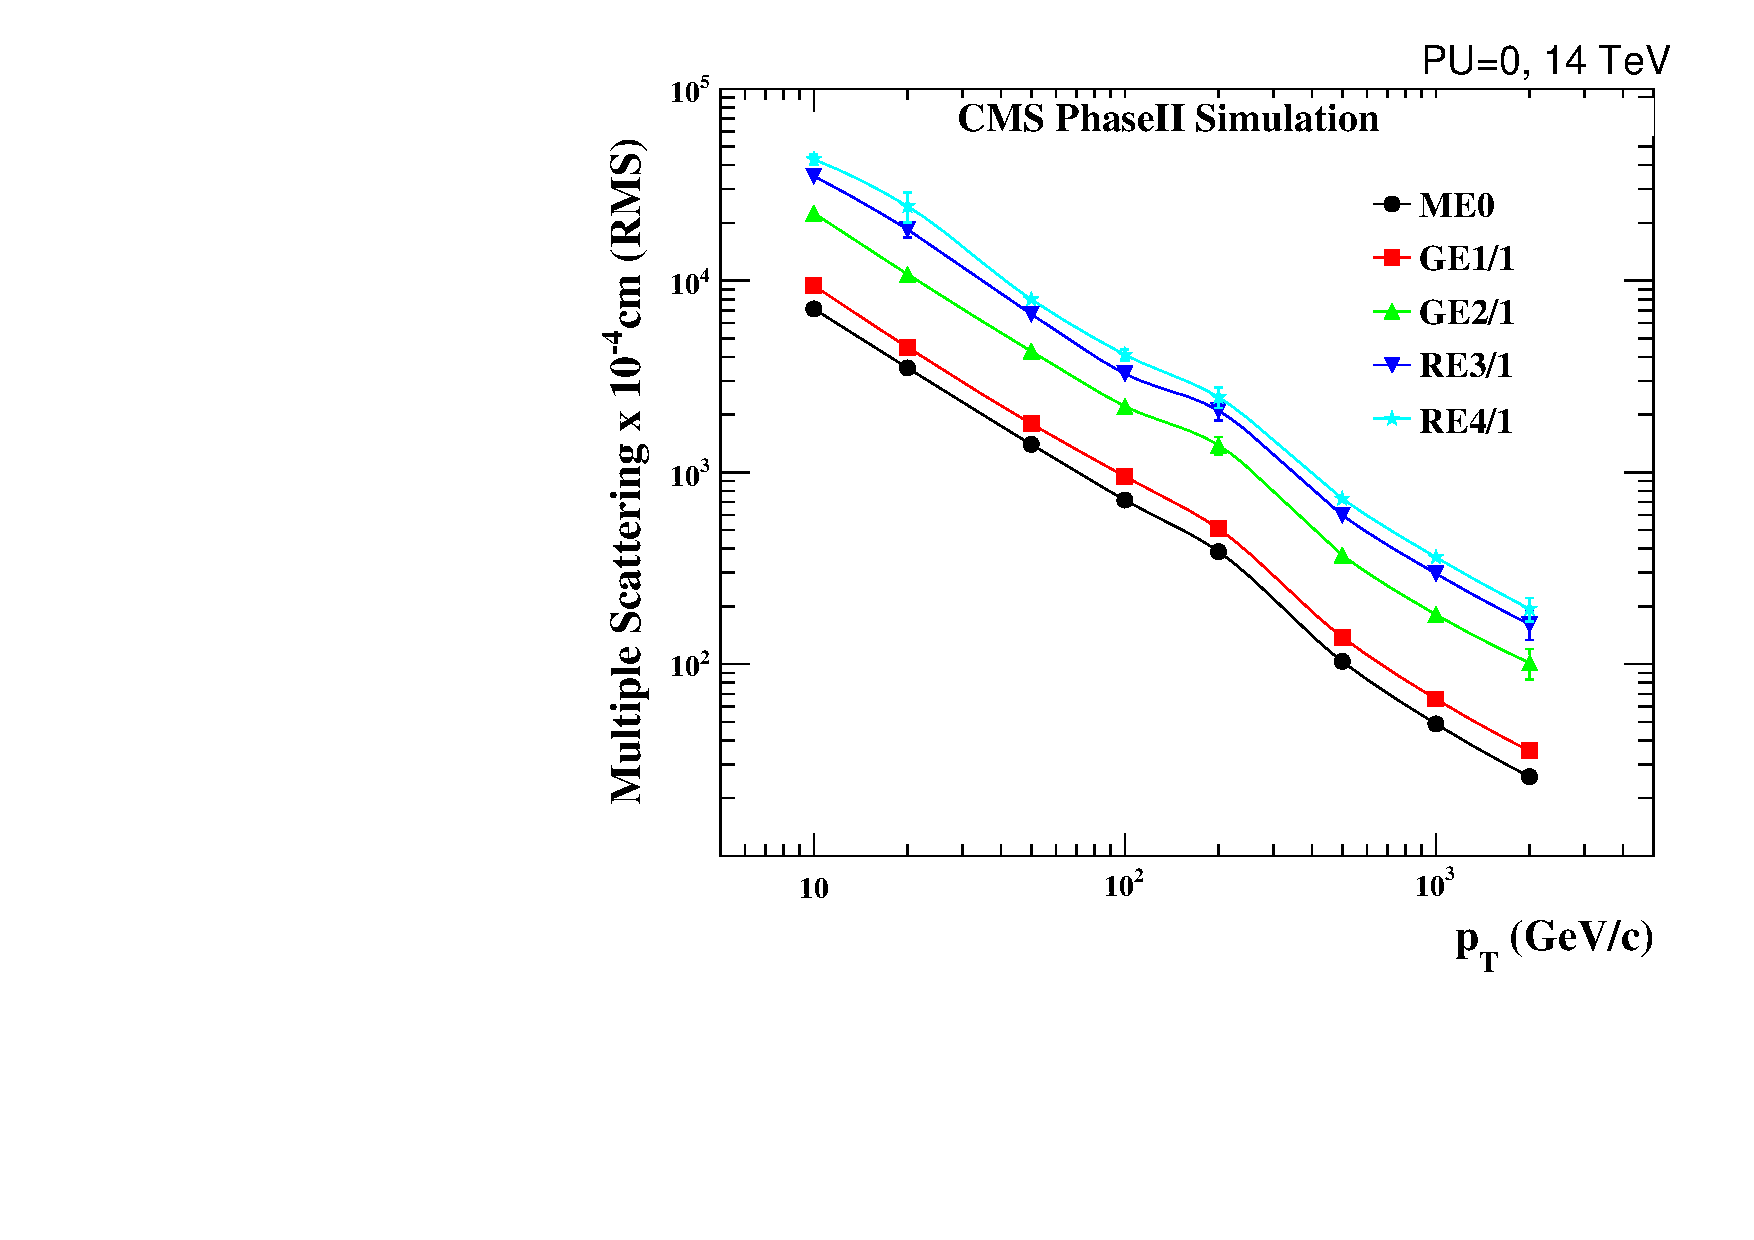
\includegraphics[width=0.6\textwidth]{fig/chapt2/MS_allstations.pdf}
	\caption{\label{fig:MultiScat}  RMS of the multiple scattering displacement as a function of muon $p_T$ for the  proposed forward muon stations. All of the electromagnetic processes such as bremsstrahlung and magnetic field effect are included in the simulation.}
\end{figure}

\clearpage{\pagestyle{empty}\cleardoublepage}
